\section{变分方法与数据拟合}
\subsection{绪论}
  若要求函数$\f(\mbf{x})$,$x\in\R^n$的最值点,根据
  Fermat引理,只需要求出所有成立$\nabla\f = 0$的点再
  逐一验证即可. 变分是这一思想的推广,它所处理的是过程的优化.
  下给出一个优化过程的例子,完整的解答见之后的章节. (todo: ref)

  \begin{exa}[最速降线]
    给定空中的一点$A=(0,0)$,地上一点$B=(x_1,y_1)$,求一条连接
    $A$和$B$的轨迹,使得假设在无阻力情况下,有小球沿轨道从$A$到$B$
    所需要的时间最短. \par
    假设轨道曲线充分光滑,则问题可以转换为,设滑行轨道$y\in\ms{C}^2$的方程为
    \[
      y=y(x), \quad y(0)=0,\quad y(x_1) = y_1.
    \]
    试确定曲线$y$使得时间$T(y)$最小. 根据机械能守恒,小球在$(*,-y)$处
    (见\figref{fig: 最速降线问题})的速度,为
    \[
      v = \sqrt{2gy},
    \]
    同时由速度的定义知
    \[
      v = \frac{\rd s}{\rd t} = \sqrt{1+y^{\pr2}(x)}\frac{\rd x}{\rd t},
    \]
    根据上两式,即有
    \[
      \sqrt{2gy}\rd t = \sqrt{1+y^{\pr2}(x)}\rd x \,\Rightarrow\,
      \rd t = \left( \frac{1+y^{\pr2}}{2gy} \right)^{1/2}\rd x
    \]
    设过程为$A\to B$,$0\to t_1$,$0\to x_1$,则
    \[
      T(y) = t_1 = \int_0^{x_1} \left( \frac{1+y^{\pr2}}{2gy} \right)^{1/2}\rd x,
    \]
    即为所要最小化的$T(y)$.
    \begin{figure}[htbp]
      \centering
      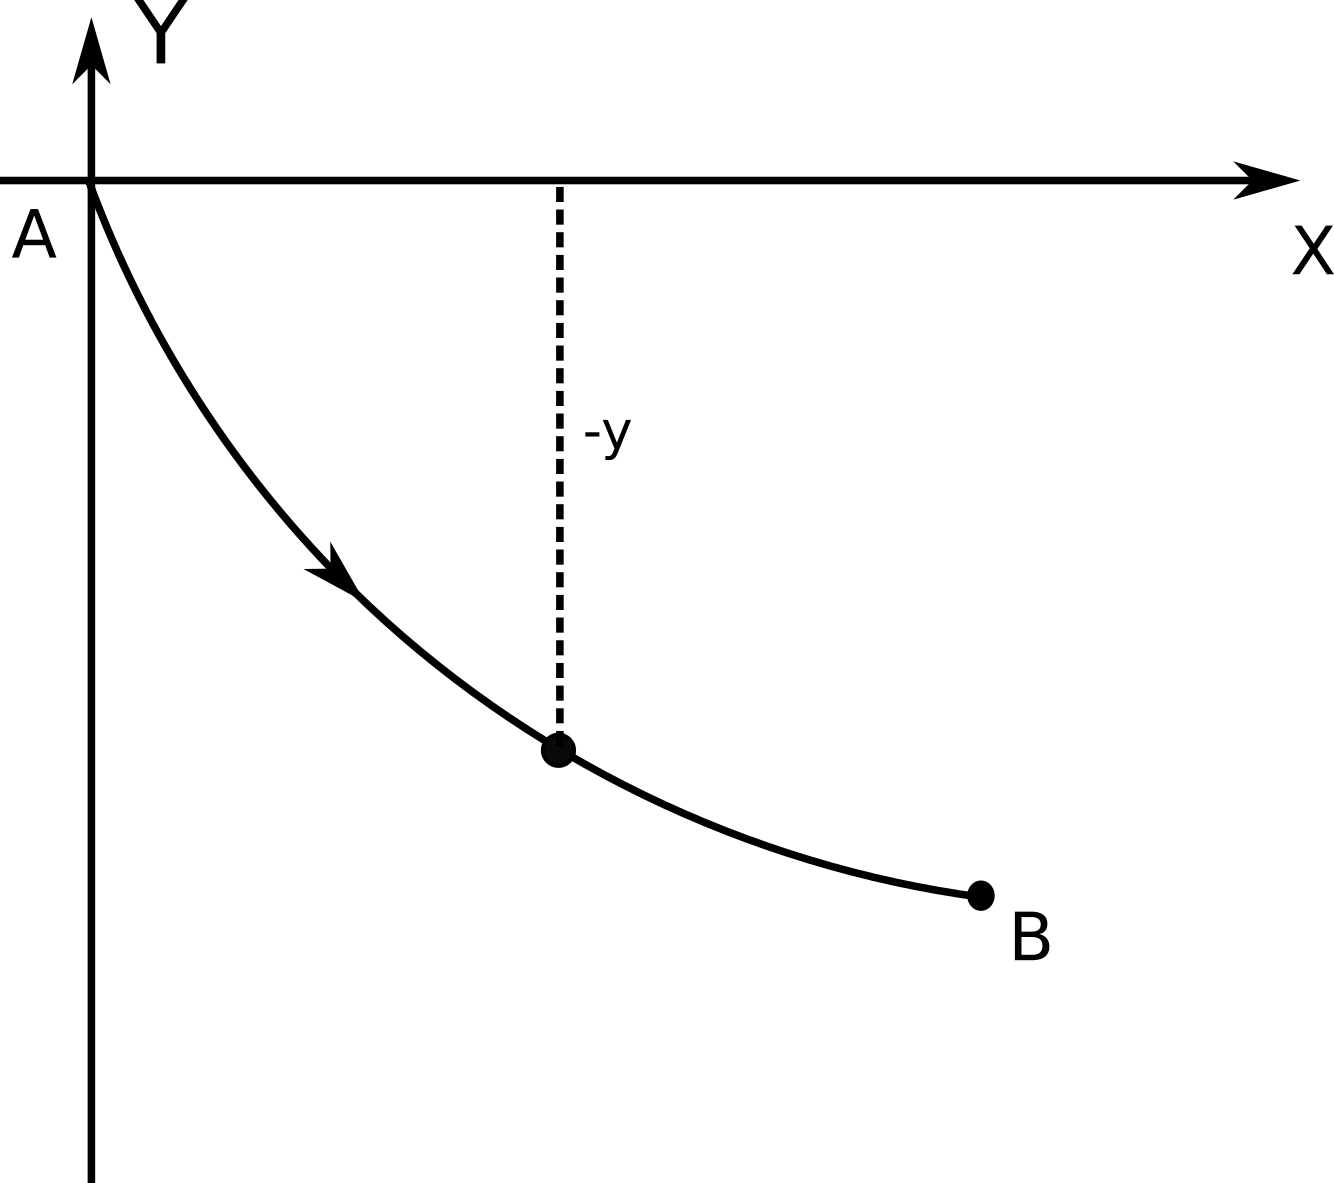
\includegraphics[height=5cm]{../image/brachistochrone.png}
      \caption{最速降线问题}
      \label{fig: 最速降线问题}
    \end{figure}
  \end{exa}

\newpage
\subsection{变分方法}
  \begin{defi}[过程优化]
    \label{def: 过程优化}
    过程的优化即求解
    \[
      \label{equ: 过程优化}
      y^* = \agm_{y\in K}J(y)
    \]
    的过程,其中函数集合
    \[
      K = \{y\in\ms{C}^2[x_0, x_1]\,:\, y(x_0)=y_0,\,y(x_1)=y_1\}.
    \]
  \end{defi}

  \begin{defi}
    \label{defi: K}
    定义函数集合
    \[\begin{split}
      K &= \{\f\in\ms{C}^2[x_0, x_1]\,:\,\f(x_0)=y_0,
      \f(x_1) = y_1\}, \\
      K_0 &=\{\f\in\ms{C}^2[x_0, x_1]\,:\,\f(x_0)=
      \f(x_1) = 0\}.
    \end{split}\]
    对于任意$\f_0\in K$,$\eta \in K_0$定义集合
    \[
      K(\f_0, \eta) = \{\f_0 + \vep\eta\,:\,\vep\in\R\}.
    \]
  \end{defi}

  \begin{defi}[泛函的方向导数]
    \label{def: 泛函的方向导数}
    记号同\defref{defi: K}. 定义泛函
    \[
      J(\f) = \int_a^bL(x, \f(x), \f\hp(x)) \rd x,\quad
      \f \in K.
    \]
    如果$\f^*$是函数$J(\f)$在集合$K$中的最小值点,即
    \[
      \f^* = \agm_{\f\in K}J(\f),
    \]
    则对于任意$\eta\in K_0$,$\f^*$也是$J(\f)$在集合$K(\f^*,\eta)$
    中的最小值点. 所以成立
    \[
      \f^* = \agm_{\vep\in\R}J(\f^* + \vep\eta).
    \]
    由于函数$J(\f^* + \vep\eta)$是关于实数$\vep$的一元函数,所以在
    它最小值点,即$\vep =0$处成立
    \begin{equation}
      \label{equ: 方向导数为零}
      \frac{\rd}{\rd\vep}J(\f^* + \vep\eta)\bigg|_{\vep =0}=0.
    \end{equation}
    称左侧为泛函$J$在$\f^*$处沿$\eta$方向的\tbf{变分}
    或\tbf{方向导数}. 即为$\delta J(\f^*, \eta)$\footnote{一般来讲,
    $\f^*$可以是集合中的任意一点. }.
  \end{defi}
  \remark
    这里采用的是分析学中一个常见思想,将一个在高维空间中的问题
    转化为一个低维空间中的问题. 一个更加简单的例子是,证明若
    $k$维欧式空间中的函数$\f$在凸集$K$中的各偏导数恒为零,则
    它在$K$中为常量. 一个证法是取定$K$中任意一点(向量)$\mbf{x}_0$,
    则对于任意$\mbf{x}\in K$,则对于任意直线段$xx_0$,有方程
    \[
      y = \mbf{x_0}t + \mbf{x}(1-t).
    \]
    上式是一个一元实函数,对它求导并利用一元函数微分学中的知识,可以
    知道在这条直线段上$\f$的函数值不变. 由于$\mbf{x}_0$和$\mbf{x}$
    的选取是任意的,所以在$K$上$\f$的值不变. \par
    在这里采用的是同样的思想,只是把欧式空间换成了一个函数集合而已.

  \begin{lemma}[变分引理 I]
    \label{lemma: 变分引理}
    设$\f\in\ms{C}[a,b]$,且对任意满足$\g(a)=\g(b)=0$的
    $\g\in\ms{C}^2[a,b]$,有
    \[
      \int_{a}^{b}\f\g \rd x =0,
    \]
    则在$[a,b]$上成立$\f\equiv 0$.
  \end{lemma}

  \begin{lemma}[变分引理 II]
    设$\f\in\ms{C}[a, b]$,且对于任意满足$\eta(a) = \eta(b) = 0$的
    $\eta\in\ms{C}^1(a, b)$都成立
    \[
      \int_a^b\f\eta\hp\rd x = 0,
    \]
    则在$[a, b]$上成立$\f\equiv \text{Const}$.
  \end{lemma}

  \begin{thm}[Euler-Lagrange方程]
    \label{thm: Euler-Lagrange方程}
    记号同\defref{def: 泛函的方向导数}. 泛函$J(\f)$在极值点满足
    Euler-Lagrange方程
    \begin{equation}
      \label{equ: Euler-Lagrange方程}
      \frac{\partial L}{\partial\f} - \frac{\rd}{\rd x}\frac{\partial L}{\partial\f\hp} = 0.
    \end{equation}
  \end{thm}
  \proof
    假设满足求导积分换序的条件,则泛函$J(\f)$在
    $\f_*+\vep\eta$处沿$\eta$方向的方向导数为
    \footnote{为了记号的清晰,这里用$\f_*$替代之前的$\f^*$.
    并且这里关于偏导数的记号,应理解为关于分母所表示的那一分量的偏导数. }
    \[\begin{split}
      \frac{\rd}{\rd\vep}J(\f_*+\vep\eta) &=
      \frac{\rd}{\rd\vep}\int_{x_0}^{x_1}L(x,\f_*+\vep\eta,\f_*\hp+\vep\eta\hp)\rd x\\
      &= \int_{x_0}^{x_1} \frac{\partial L}{\partial (\f_*+\vep\eta)}\eta
      +\frac{\partial L}{\partial (\f_*\hp+\vep\eta\hp)}\eta\hp\,\rd x.
    \end{split}\]
    代入$\vep=0$,即得$J$在最小值点$\f_*$处的方向导数,为
    \[\begin{split}
      \frac{\rd}{\rd\vep}J(\f_*) &=
      \int_{x_0}^{x_1} \frac{\partial L}{\partial \f}\eta
      +\frac{\partial L}{\partial \f\hp}\eta\hp\,\rd x \\
      &= \int_{x_0}^{x_1} \frac{\partial L}{\partial\f}\eta\rd x
      + \frac{\partial L}{\partial\f\hp}\eta\bigg|_{x_0}^{x_1}
      - \int_{x_0}^{x_1}\eta\frac{\rd}{\rd x}\frac{\partial L}{\partial \f\hp}\rd x\\
      &= \int_{x_0}^{x_1} \eta\left( \frac{\partial L}{\partial\f}
      - \frac{\rd}{\rd x}\frac{\partial L}{\partial\f\hp} \right) \rd x = 0.
    \end{split}\]
    注意由于$\eta\in K_0$,即有$\eta(x_0) = \eta(x_1) = 0$.
    由于$\eta$的选取是任意的,所以根据\lemmaref{lemma: 变分引理},式子
    \equref{equ: Euler-Lagrange方程}成立. $\blacksquare$
  \remark
    对于$L = L(\f,\f\hp)$,即$L$不显含$x$的情况,
    \equref{equ: Euler-Lagrange方程}是可以精确求解的.

  \begin{thm}[守恒律定理]
    \label{thm: 守恒律定理}
    设$L = L(\f,\f\hp)$,则沿着\equref{equ: 过程优化}的解曲线
    $y^* = \f^*(x)$,成立
    \[
      H = \f\hp\frac{\partial L}{\partial\f\hp} - L = \text{Const}.
    \]
  \end{thm}
  \proof
    \[\begin{split}
     \frac{\rd H}{\rd x} &= \frac{\rd}{\rd x}
     \left( \f\hp\frac{\partial L}{\partial\f\hp}-L(\f,\f\hp) \right)\\
     &= \f^{\pr\pr}\frac{\partial L}{\partial\f\hp}
     + \f\hp\frac{\rd}{\rd x}\frac{\partial L}{\partial\f\hp} -
     \frac{\partial L}{\rd\f}\f\hp -
     \frac{\partial L}{\rd\f\hp}\f^{\pr\pr}.
    \end{split}\]
    根据\thmref{thm: Euler-Lagrange方程},$\rd H /\rd x =0$,所以
    命题成立. $\blacksquare$

  % \begin{exa}[最速降线的求解]
  %   根据之前的讨论,即求解
  %   \[
  %     \f_* = \agm_{\f\in K} T(\f) = \int_{0}^{x_1}
  %     \left( \frac{1+\f\hp}{2g\f} \right)^{1/2}\rd x.
  %   \]
  %   根据\thmref{thm: 守恒律定理},成立
  %   \[
  %
  %   \]
  % \end{exa}

\newpage
\subsection{曲线拟合的正则化方法}
  \begin{defi}[Tikhonov正则化]
    \label{def: Tikhonov正则化}
    对于给定的数据$Y$,定义数据拟合项为$J_1(\f)$,用于表示拟合结果
    相较于原数据的接近程度,同时要求拟合的结果尽可能满足对于结果的
    要求,用$J_2(\f)$来描述$\f$满足要求的程度,则求解拟合结果的
    过程即为求解
    \[
      \f_* = \agm_{\f\in K}(J_1(\f) + \alpha J_2(\f)).
    \]
    其中$\alpha$为\tbf{正则化参数},用于表示拟合的过程中,应更接近
    原数据或是更满足拟合要求. 若取$\alpha=0$,即为插值.
  \end{defi}

  \begin{prob}
    给定函数$y$在样本点$0=x_0 < x_1 < \cdots < x_n = 1$处的
    近似值$\tilde{y}_i$,误差满足
    \[
      |\tilde{y}_i - y(x_i)| \le \delta,
    \]
    试重构$y$的近似函数$\f_*$.\par
    按照\defref{def: Tikhonov正则化}的思想,定义
    \[\begin{split}
      J_1(\f) &= \sum_{i=1}^{n-1}\frac{h_i+h_{i+1}}{2}
      \left( \tilde{y}_i - \f(x_i) \right)^2 \\
      J_2(\f) &= \int_0^1 (\f^{\pr\pr})^2\rd x
    \end{split}\]
    其中
    \[\begin{split}
      h_i &= x_i - x_{i-1},\quad i = 1,2,\dots,n\\
      h &= \max_{1\le i\le n}h_i
    \end{split}\]
    则问题转换为求解
    \begin{equation}
      \label{equ: 正则化曲线拟合}
      \f_* = \agm_{\f\in K}\left( J_1(\f) + \alpha J_2(\f) \right).
    \end{equation}
  \end{prob}
  \remark
    不失一般性的,可以设$\tilde{y}_0 = \f(x_0)$且$\tilde{y}_n=\f(x_n)$.
    否则只需要用
    \[
      Y(x) = y(x)+\tilde{y}_0-y(0)+(\tilde{y}_n-y(1)+y(0)-\tilde{y}_n)x
    \]
    来替代$y$即可. 可以证明
    \begin{enumerate}
      \item $Y(0) = \tilde{y}_0$且$Y(1) = \tilde{y}_n$,
      \item $|\tilde{y}_i - Y(x_i)| \le 4\delta$.
    \end{enumerate}

  \begin{thm}
    对于任意$\alpha>0$,\equref{equ: 正则化曲线拟合}的解为三次样条函数.
  \end{thm}
  \proof
    设$\f_*$为式\equref{equ: 正则化曲线拟合}的解. \par
    对于任意$\eta\in K_0$,$\vep\in R$,
    \[
      J(\f_*+\vep\eta) = \sum_{i=1}^{n-1}\frac{h_i + h_{i+1}}{2}
      [\tilde{y}_i - f_*(x_i) - \vep\eta(x_i)]^2 + \alpha
      \int_0^1(\f_*^{\pr\pr} + \vep\eta^{\pr\pr})^2\,\rd x.
    \]
    求它关于$\vep$的导数,成立
    \[
      \frac{\rd}{\rd\vep}J(\f_*+\vep\eta) =
      -2\sum_{i=1}^{n-1}\frac{h_i+h_{i+1}}{2}[\tilde{y}_i-\f_*(x_i)-\vep\eta(x_i)]\eta(x_i)
      +2\alpha\int_0^1 (\f_*^{\pr\pr}+\vep\eta^{\pr\pr})\eta^{\pr\pr} \,\rd x.
    \]
    根据\defref{def: 泛函的方向导数}中的\equref{equ: 方向导数为零},上式在$\vep=0$时
    值为零,即
    \begin{equation}
      \label{equ: 正则化证明1}
      \frac{\rd}{\rd\vep}J(\f_*+\vep\eta)\bigg|_{\vep=0} =
      -2\sum_{i=1}^{n-1}\frac{h_i+h_{i+1}}{2}[\tilde{y}_i-\f_*(x_i)]\eta(x_i)
      +2\alpha\int_0^1\f_*^{\pr\pr}\eta^{\pr\pr}\,\rd x = 0.
    \end{equation}
    接下来分两步构造出$\f_*$.\\
  \tbf{Step 1. }
    由于$\eta$的选取是任意的,所以我们选择恰当的$\eta\in\ms{C}^\infty(x_i,x_{i+1})$,
    使得成立
    \[
      \eta(x_i) = 0,\quad i = 1,2,\dots,n-1
    \]
    所以根据\equref{equ: 正则化证明1},成立
    \[
      \int_{x_i}^{x_{i+1}}\f_*^{\pr\pr}\eta^{\pr\pr} = 0.
    \]
    对于上式进行两次分部积分,得到
    \[
      0 = \f_*^{\pr\pr}\eta\hp\bigg|_{x_i}^{x_{i+1}} -
      \f_*^{(3)}\eta\bigg|_{x_i}^{x_{i+1}} +
      \int_{x_i}^{x_{i+1}}\f_*^{(4)}\eta\rd x.
    \]
    同样因为$\eta$的选取是任意的,所以可以在原来的基础上,选取$\eta$使得成立
    \[
      \eta(x_i) = \eta\hp(x_i) = 0,\quad i = 1,2,\dots,n-1
    \]
    所以有
    \[
      \int_{x_i}^{x_{i+1}}\f_*^{(4)}\eta\rd x = 0.
    \]
    根据变分引理,即成立
    \begin{equation}
      \label{equ: 正则化证明2}
      \f_*^{(4)}(x) = 0\quad\Rightarrow\quad \f\in P_3,\quad x\in(x_i,x_{i+1}).
    \end{equation}
  \tbf{Step 2. }
    取满足$\eta(0)=\eta(1)=0$的$\eta\in\ms{C}^\infty[0, 1]$,分部积分得
    (注意$\f_*^{(4)} = 0$)
    \[\begin{split}
      \int_0^1 \f_*^{\pr\pr}\eta^{\pr\pr}\rd x =&
      \sum_{i=1}^{n-1}
      \left(
        -\f_*^{(3)}\eta\bigg|_{x_i-1}^{x_i}
        +\f_*^{\pr\pr}\eta\hp\bigg|_{x_i-1}^{x_i}
      \right) \\
      =& \sum_{i=1}^{n-1}
      ( \f_*^{(3)}(x_i+) - \f_*^{(3)}(x_i-))\eta(x_i) +
      \sum_{i=1}^{n-1} ( \f_*^{\pr\pr}(x_i+) - \f_*^{\pr\pr}(x_i-))\eta\hp(x_i)\\
      & + \f_*^{\pr\pr}(1)\eta\hp(1) - \f_*^{\pr\pr}(0)\eta\hp(0)
    \end{split}\]
    将结果带入\equref{equ: 正则化证明1},即
    \begin{equation}\begin{split}
      \label{equ: 正则化证明3}
      0 =&
      \f_*^{\pr\pr}(1)\eta\hp(1) - \f_*^{\pr\pr}(0)\eta\hp(0)\\
      &+\sum_{i=1}^{n-1} \left(
        -\frac{h_i+h_{i+1}}{2}[\tilde{y}_i - \f_*(x_i)]
        + \alpha(\f_*^{(3)}(x_i+) - \f_*^{(3)}(x_i-))
      \right)\eta(x_i) \\
      &+\alpha\sum_{i=1}^{n-1} ( \f_*^{\pr\pr}(x_i+) - \f_*^{\pr\pr}(x_i-))\eta\hp(x_i)
    \end{split}\end{equation}
    由于$\eta$的选取是任意的,即意味着$\eta(x_i)$,$(i=1,2,\dots,n-1)$和
    $\eta\hp(x_i)$,$(i=0,1,\dots,n)$的选取是任意的,所以需要选取适当的$\f$才可以使得
    \equref{equ: 正则化证明3}中的每一项都恒为零. 为使第$1$、$3$项为零,需要满足
    \[\begin{split}
      & \f_*^{\pr\pr}(1) = \f^{\pr\pr}(0) = 0,\\
      & \f_*^{\pr\pr}(x_i+) = \f_*^{\pr\pr}(x_i-).
    \end{split}\]
    同样的,根据不同的$\alpha$,选取恰当的$\f(x_i)$或
    $\f^{(3)}(x_i)$使得第二项为零.
    综合上式以及\equref{equ: 正则化证明2},可知$\f_*$为三次样条函数,
    且当$\alpha=0$时为样条插值函数. $\blacksquare$
